%%%%%%%%%%%%%%%%%%%%%%%%%%%%%%%%%%%%%%%%%%%%%%%%%%%%%%%%%%%
% --------------------------------------------------------
% Tau
% LaTeX Template
% Version 2.4.4 (28/02/2025)
%
% Author: 
% Guillermo Jimenez (memo.notess1@gmail.com)
% 
% License:
% Creative Commons CC BY 4.0
% --------------------------------------------------------
%%%%%%%%%%%%%%%%%%%%%%%%%%%%%%%%%%%%%%%%%%%%%%%%%%%%%%%%%%%

\documentclass[9pt,a4paper,twocolumn,twoside]{tau-class/tau}
\usepackage[portuguese]{babel}

%% Spanish babel recomendation
% \usepackage[spanish,es-nodecimaldot,es-noindentfirst]{babel} 

%% Draft watermark
% \usepackage{draftwatermark}

%----------------------------------------------------------
% TITLE
%----------------------------------------------------------

\journalname{Universidade de Fortaleza (Unifor) - Pós-Graduação em Informática Aplicada}
\title{Relatório de Laboratório 2025.S1-E1.01}

%----------------------------------------------------------
% AUTHORS, AFFILIATIONS AND PROFESSOR
%----------------------------------------------------------

\author[a,1]{Jonas de Araújo Luz Junior}
\author[a,2]{José de La Cruz Iraheta}
\author[a,3]{Pedro Jardelino Neto}

%----------------------------------------------------------

\affil[a]{Universidade de Fortaleza (Unifor)}
%\affil[b]{Affiliation of author two}
%\affil[c]{Affiliation of author three}

\professor{Professor Nabor das Chagas Mendonça}

%----------------------------------------------------------
% FOOTER INFORMATION
%----------------------------------------------------------

\institution{Universidade de Fortaleza (Unifor)}
\footinfo{Disciplina: M-907 - Sistemas Distribuídos}
\theday{06 de maio de 2025}
\leadauthor{Luz Jr., J.A.; Iraheta, J.L.C.; and Neto, P.J.}
\course{Creative Commons CC BY 4.0}

%----------------------------------------------------------
% ABSTRACT AND KEYWORDS
%----------------------------------------------------------

\begin{abstract}    
Este relatório descreve a execução da \textbf{Primeira Entrega Parcial} do trabalho
prático proposto no Laboratório de Sistemas Distribuídos, cujo objetivo é
provisionar um cluster Kubernetes local, instalar o service‑mesh Istio e
implantar a aplicação de micro‑serviços \emph{Online Boutique}.
\end{abstract}

%----------------------------------------------------------

\keywords{Relatório de laboratório, Sistemas distribuídos, Kubernetes, Istio, Docker}

%----------------------------------------------------------

\begin{document}
		
    \maketitle 
    \thispagestyle{firststyle} 
    \tauabstract 
    % \tableofcontents
    % \linenumbers 
    
%----------------------------------------------------------

\section{Especificação da Entrega}

\subsection{Tarefa 1 - Configuração do Ambiente}
\begin{itemize}
    \item Configurem um repositório Git compartilhado para o projeto.
    \item Instalem e configurem a distribuição Kubernetes local escolhida em suas máquinas (ou em uma máquina compartilhada pela equipe). Certifiquem-se de alocar recursos suficientes (CPU/RAM).
    \item Instalem o Istio no cluster Kubernetes, utilizando o perfil de instalação demo ou default. Verifiquem a instalação.
\end{itemize}

\subsection{Tarefa 2 - Implantação da Aplicação}
\begin{itemize}
    \item Obtenham os manifestos de implantação da aplicação Online Boutique.
    \item \textbf{\textit{Implantação base:}} implantem a aplicação sem a injeção automática de sidecars do Istio (ou seja, em um namespace sem o rótulo \texttt{istio-injection=enabled}). Verifiquem se todos os serviços estão rodando e se a aplicação está acessível .
    \item \textbf{\textit{Implantação com Istio:}} habilitem a injeção automática de sidecars do Istio para um novo namespace (e.g., \texttt{online-boutique-istio}) e implantar a aplicação novamente neste namespace. Verifiquem se os sidecars foram injetados (\texttt{kubectl get pods -n -o wide} deve mostrar 2/2 containers por pod) e se a aplicação continua acessível.
\end{itemize}

\subsection{Entregáveis:}
\begin{enumerate}
    \item Relatório Preliminar (2-3 páginas) \textit{[este]} incluindo:
    \begin{enumerate}
        \item Formação da equipe e link para o repositório Git criado.
        \item Evidência do sucesso (e.g., screenshots, logs) na instalação e configuração do ambiente Kubernetes local (incluir versão, recursos alocados).
        \item Evidência do sucesso (e.g., screenshots, logs) na instalação do Istio (incluir versão, perfil utilizado).
        \item Evidência do sucesso (e.g., screenshots, logs) na implantação da aplicação Online Boutique nos dois cenários (sem e com injeção do sidecar Istio).
        \item Repositório Git atualizado com a estrutura inicial e quaisquer scripts/manifestos básicos utilizados.
    \end{enumerate}
\end{enumerate}

%----------------------------------------------------------

\section{Repositório Git}
\begin{itemize}[leftmargin=*]
  \item Repositório oficial do projeto (código, manifestos, evidências):\\
  \url{https://github.com/jonasluz/DIA.kubernetes-istio/}
\end{itemize}

%----------------------------------------------------------

\section{Ambiente de Trabalho}
\begin{description}[leftmargin=1.5cm]
  \item[Sistema] Fedora 41 (x86\_64) atualizado em \today.
  \item[Recursos] 8 GB RAM, 4 vCPU, 60 GB SSD.
  \item[Container Runtime] Docker \texttt{24.x} (moby‑engine) \cite{docker}.
  \item[Cluster] Minikube \texttt{v1.35.0} com Kubernetes \texttt{v1.32.0} \cite{minikube}.
  \item[Istio] \texttt{1.22.0} (perfil \texttt{demo}) \cite{istio}.
\end{description}

% -----------------------------------------------------------------------------
\section{Passo a Passo da Instalação}
\label{sec:passoapasso}
Os comandos abaixo foram executados sequencialmente em shell \texttt{bash}. Cada
etapa inclui uma breve explicação e um espaço reservado para evidência (log ou
captura de tela).

\subsection{Atualização do Sistema}
\begin{enumerate}[label=\arabic*.]
  \item \textbf{Atualizar pacotes e utilitários básicos}
\begin{lstlisting}[language=Bash]
sudo dnf upgrade --refresh -y && sudo reboot
\end{lstlisting}
    after reboot:
\begin{lstlisting}[language=Bash]
sudo dnf install -y curl wget git conntrack jq
\end{lstlisting}
\end{enumerate}

\subsection{Instalação do Docker}
\begin{enumerate}[label=\arabic*.]
    \item\textbf{Adicionar repositório Docker CE e instalar runtime}

\begin{lstlisting}[language=Bash]
sudo dnf install -y dnf-plugins-core
sudo dnf config-manager --add-repo \
  https://download.docker.com/linux/fedora/docker-ce.repo
sudo dnf install -y docker-ce docker-ce-cli containerd.io \
  docker-buildx-plugin docker-compose-plugin
sudo systemctl enable --now docker
sudo usermod -aG docker $(whoami)
\end{lstlisting}
\textit{Evidência:} Figura \ref{fig:docker}.\\

\begin{figure}[h]
    \centering
    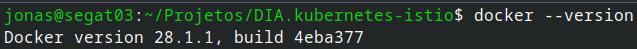
\includegraphics[width=1\linewidth]{figures/evidence-docker}
    \caption{Evidência: Instalação do Docker}
    \label{fig:docker}
\end{figure}
\end{enumerate}

\subsection{Instalação do kubectl}
\begin{enumerate}[label=\arabic*.]
\item\textbf{Baixar binário compatível (v1.32.0)} \cite{kubernetes}

\begin{lstlisting}[language=Bash]
curl -LO https://dl.k8s.io/release/v1.32.0/bin/linux/amd64/kubectl
sudo install -o root -g root -m 0755 kubectl /usr/local/bin/
rm kubectl
\end{lstlisting}
\textit{Evidência:} Figura \ref{fig:kubectl}.\\

\begin{figure}[h]
    \centering
    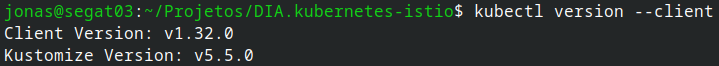
\includegraphics[width=1\linewidth]{figures/evidence-kubectl.png}
    \caption{Evidência: Instalação do kubectl}
    \label{fig:kubectl}
\end{figure}
\end{enumerate}

\subsection{Instalação do Minikube}
\begin{enumerate}[label=\arabic*.]
\item\textbf{Baixar Minikube v1.35.0} \cite{minikube}

\begin{lstlisting}[language=Bash]
curl -LO https://github.com/kubernetes/minikube/releases/download/v1.35.0/minikube-linux-amd64
sudo install minikube-linux-amd64 /usr/local/bin/minikube
rm minikube-linux-amd64
\end{lstlisting}

\item\textbf{Inicializar cluster (driver Docker)}
\begin{lstlisting}[language=Bash]
minikube start --driver=docker --cpus=4 --memory=8192
\end{lstlisting}
\textit{Evidência:} Figura \ref{fig:minikube}.\\

\begin{figure}[h]
    \centering
    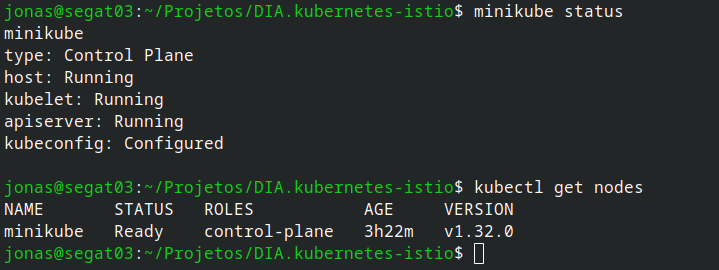
\includegraphics[width=1\linewidth]{figures/evidence-minikube.png}
    \caption{Evidência: Instalação do Minikube.}
    \label{fig:minikube}
\end{figure}
\end{enumerate}

\subsection{Instalação do Istio}
\begin{enumerate}[label=\arabic*.]
    \item\textbf{Download e instalação do Istioctl 1.22.0}
\begin{lstlisting}[language=Bash]
curl -L https://istio.io/downloadIstio | ISTIO_VERSION=1.22.0 sh -
export PATH="$PATH:$HOME/istio-1.22.0/bin"
istioctl install --set profile=demo -y
istioctl verify-install
\end{lstlisting}
\textit{Evidência:} Figura \ref{fig:istio}\\

\begin{figure}[h]
    \centering
    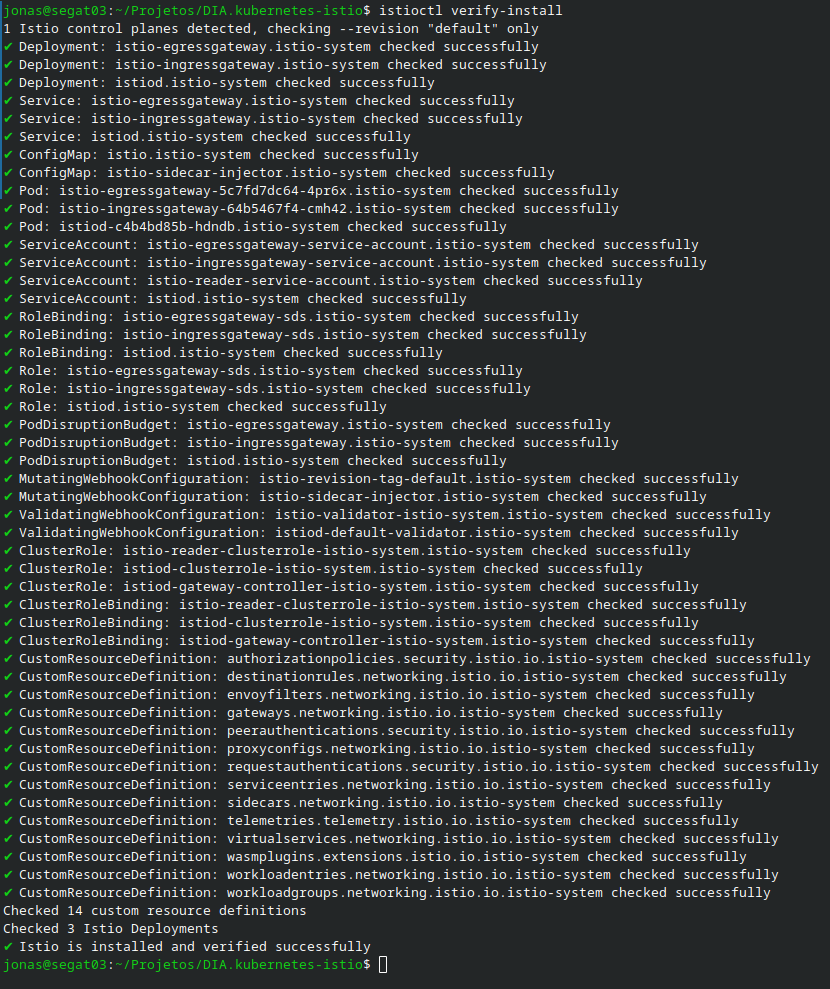
\includegraphics[width=1\linewidth]{figures/evidence-istio.png}
    \caption{Evidência: Instalação do Istio}
    \label{fig:istio}
\end{figure}
\end{enumerate}

\subsection{Implantação da Online Boutique}
\begin{enumerate}[label=\arabic*.]

\item\textbf{Clonar repositório e implantar namespace \texttt{boutique-base}} \cite{onlineboutique}.
\begin{lstlisting}[language=Bash]
git clone --depth 1 https://github.com/jonasluz/microservices-demo.git
kubectl create namespace boutique-base
kubectl apply -f microservices-demo/release/kubernetes-manifests.yaml -n boutique-base
\end{lstlisting}
\textit{Evidência:} Figuras \ref{fig:olb-istio1} e \ref{fig:olb-istio2}\\

\begin{figure}[h]
    \centering
    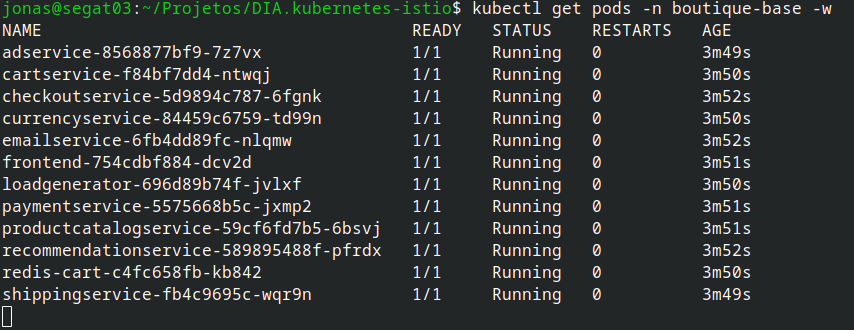
\includegraphics[width=1\linewidth]{figures/evidence-olbbase2.png}
    \caption{Evidência: Instalação da aplicação Online Boutique}
    \label{fig:olb-istio1}
\end{figure}

\begin{figure}[h]
    \centering
    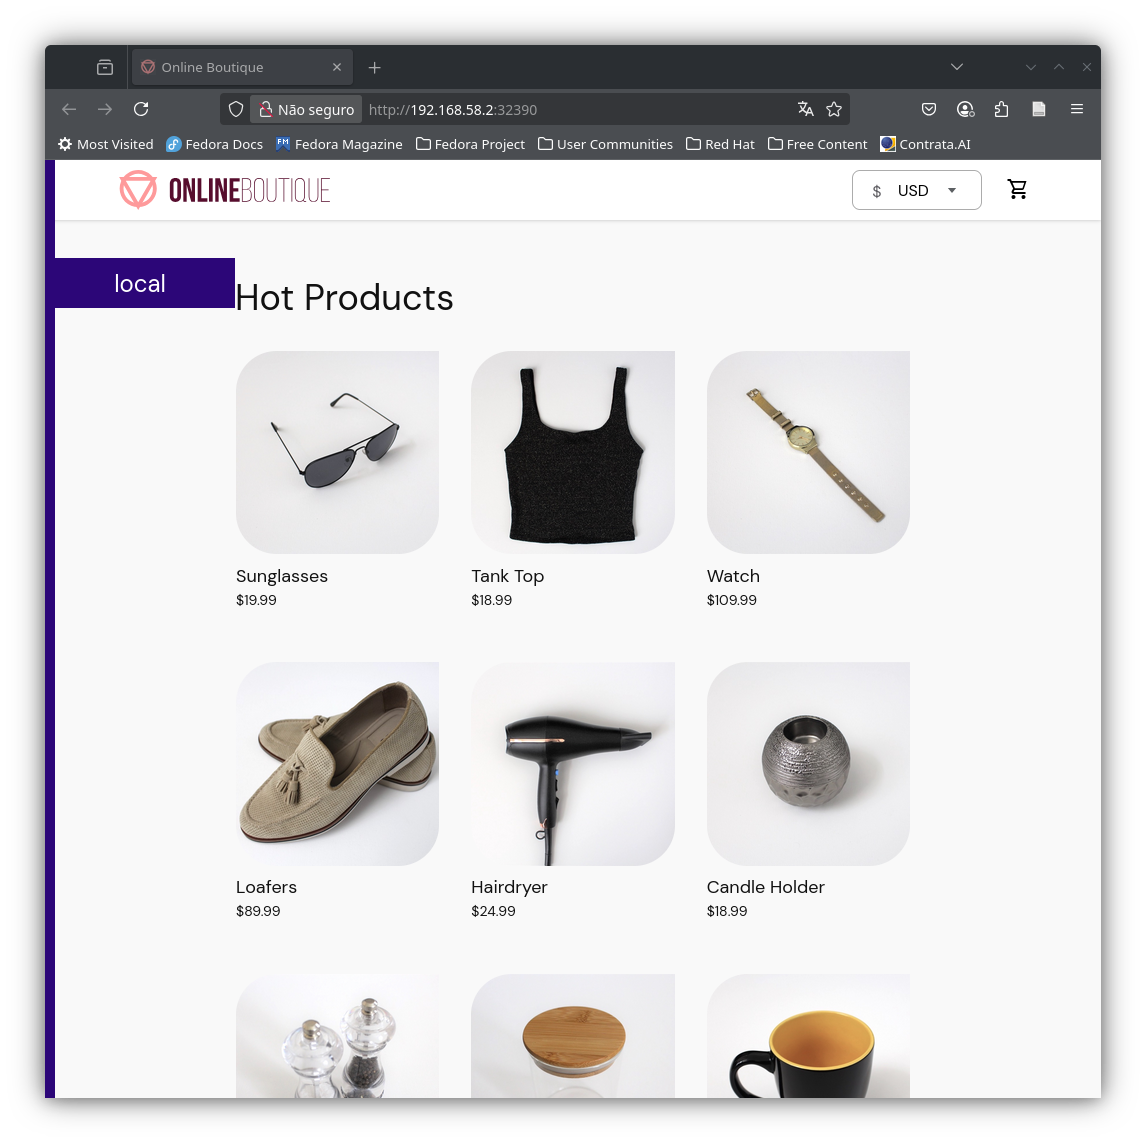
\includegraphics[width=1\linewidth]{figures/evidence-olbbase3.png}
    \caption{Evidência: Tela do navegador com a aplicação Online Boutique}
    \label{fig:olb-istio2}
\end{figure}

\item\textbf{Implantar versão com sidecars Istio (\texttt{boutique-istio})}
\begin{lstlisting}[language=Bash]
kubectl create namespace boutique-istio
kubectl label namespace boutique-istio istio-injection=enabled
kubectl apply -f microservices-demo/release/kubernetes-manifests.yaml -n boutique-istio
\end{lstlisting}
\textit{Evidência:} Figuras \ref{fig:olb-istio1} e \ref{fig:olb-istio2}\\

\begin{figure}[h]
    \centering
    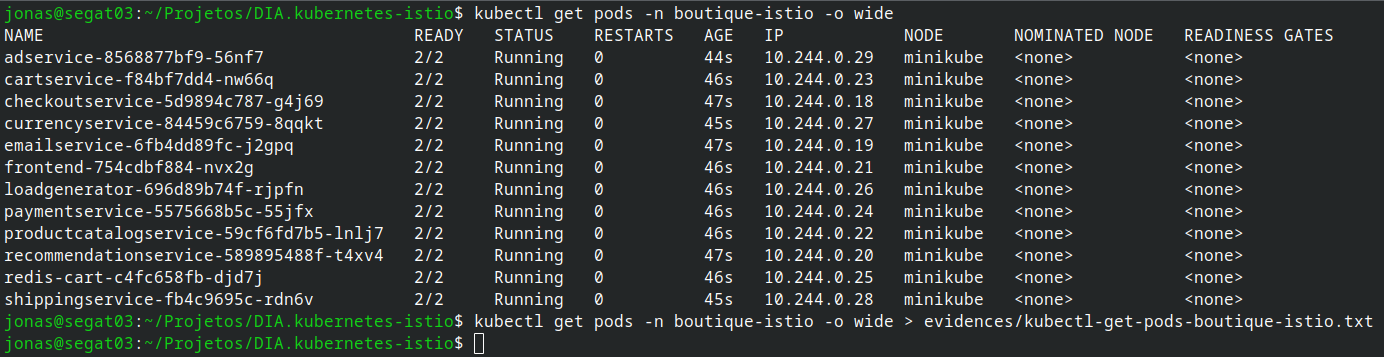
\includegraphics[width=1\linewidth]{figures/evidence-olbistio2.png}
    \caption{Evidência: Instalação da aplicação Online Boutique com Istio}
    \label{fig:olb-base1}
\end{figure}

\begin{figure}[h]
    \centering
    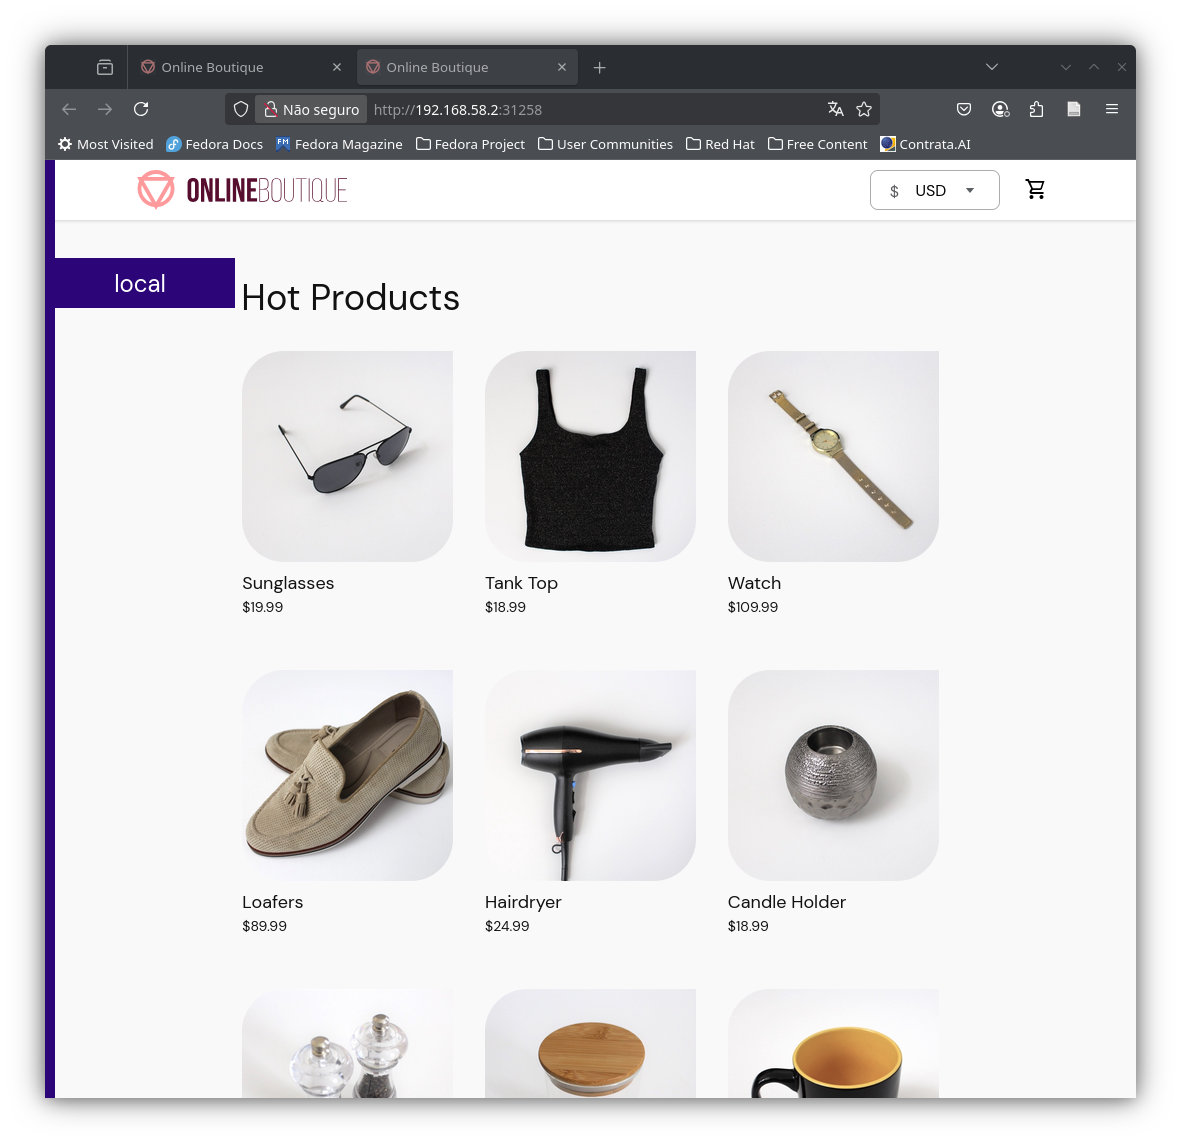
\includegraphics[width=1\linewidth]{figures/evidence-olbistio3.png}
    \caption{Evidência: Tela do navegador com a aplicação Online Boutique (com Istio)}
    \label{fig:olb-base2}
\end{figure}
\end{enumerate}

% -----------------------------------------------------------------------------
\section{Problemas Encontrados e Soluções}
\begin{itemize}[leftmargin=*]
  \item \textbf{Driver Podman rootless instável}: optou‑se pelo \emph{driver Docker}, que funcionou sem ajustes extras.
  \item \textbf{Aviso de versão do kubectl}: resolvido instalando binário 1.32.
  \item Outros problemas menores relacionados à disponibilização de pacotes e novos repositórios fonte de pacotes.
\end{itemize}

% -----------------------------------------------------------------------------
\section{Conclusão}

A primeira entrega foi concluída com êxito: cluster Kubernetes funcional em
Minikube, Istio instalado e aplicação Online Boutique implantada em dois
cenários (com e sem sidecar). As evidências coletadas encontram‑se nos espaços
reservados e em formato completo no diretório \texttt{/evidences} do
repositório oficial.

%----------------------------------------------------------

\printbibliography

%----------------------------------------------------------

\end{document}